The API is a DLL with C linkage.\par

The functions provided by the DLL are declared in \textsf{\txh{TimeTagger4}{xTDC4}{xHPTDC8}\tu interface.h}.

\section{Constants}

	\ttdef{CHANNEL\tu COUNT 4}\\
	The number of TDC input channels.\par

	 \ttdef{TIGER\tu COUNT 5}\\
	The number of timing generators. One for each TDC input and one for the \ifxHPTDC{adc trigger}{start input}.\par

	 \ttdef{TRIGGER\tu COUNT 16}\\
	The number of potential trigger sources for the timing generators. One for each TDC input, one for the Start input plus some specials. 
	 See Section~\ref{cp:tigerblock} for details.\par

\section{Initialization}
		\ttvar{int}{close(}\cronvar{\prefix device}{*device)}\\
		Finalizes the driver for this device.

		\ttvar{int}{count\tu devices(}\cronvar{int}{*error\tu code}, \cronvar{char}{**error\tu message)}\\
		Returns the number of boards present in the system that are supported by this driver.\par

		\ttvar{int}{get\tu default\tu init\tu parameters(}\cronvar{\prefix init\tu parameters}{ *init)}\\
		Sets up the standard parameters. Gets a set of default parameters for \textsf{\prefix init()}. This must always be used to initialize the \textsf{\prefix init\tu parameter()} structure.\par

		\cronvar{\prefix device *}{init(}\cronvar{\prefix init\tu parameters}{*params}, \\ \cronvar{int}{*error\tu code}, \cronvar{char}{**error\tu message)}\\
		Opens and initializes the \deviceName\ board with the given index. 
		With \textsf{error\tu code} and \textsf{error\tu message} the user must provide pointers to buffers where error information should be written by the driver.\par

		Params is a structure of type \textsf{\prefix init\tu parameters} that must be completely initialized.\par

		\subsection{Structure \prefix init\tu parameters}
			\cronvar{int}{version}\\
			The version number. Must be set to \textsf{\PREFIX API\tu VERSION}.\par

			\cronvar{int}{card\tu index}\\
			The index in the list of \deviceName\ boards that should be initialized.\\
			There might be multiple boards in the system that are handled by this driver as reported by \textsf{\prefix count\tu devices}. This index selects one of them. Boards are enumerated depending on the PCIe slot. 
			The lower the bus number and the lower the slot number the lower the card index.\par

			\cronvar{int}{board\tu id}\\
			the global index in all cronologic devices.\\
			This 8 bit number is filled into each packet created by the board and is useful if data streams of multiple boards will be merged. If only \deviceName\ cards are used this number can be set to the \textsf{card\tu index}. 
			If boards of different types that use a compatible data format are used in a system each board should get a unique id.
			Can be changed with \textsf{int \prefix set\tu board\tu id\allowbreak(\prefix device *device, int board\tu id)}.\par

			\cronvar{\tu \tu int64}{buffer\tu size[8]}\\
			The minimum size of the DMA buffer.\\
			If set to 0 the default size of 16~MByte is used. For the \deviceName\ only the first entry is used.\par

			\cronvar{int}{buffer\tu type}\\
			The type of buffer. Must be set to 0.
			\begin{description}
				\item[]  \ttdef{BUFFER\tu ALLOCATE   0}
				\item[]  \ttdef{BUFFER\tu USE\tu PHYSICAL   1}  // unsupported
			\end{description}

			\cronvar{\tu \tu int64}{buffer\tu address}\\
			This is set by \prefix init() to the start address of the reserved memory.\\ 
			The buffers will be allocated with the sizes given above. Make sure that the memory is large enough.\par

			\cronvar{int}{variant}\\
			Set to 0. Can be used to activate future device variants such as different base frequencies.\par

			\cronvar{int}{device\tu type}\\
			A constant for the different devices of cronologic \textsf{CRONO\tu DEVICE\tu *}.\\
			Initialized by \textsf{\prefix get\tu default\tu init\tu parameters()}. Must be left unchanged.
			\begin{itemize}
				\item[] \crondef{CRONO\tu DEVICE\tu HPTDC 1}
				\item[] \crondef{CRONO\tu DEVICE\tu NDIGO5G 2}
				\item[] \crondef{CRONO\tu DEVICE\tu NDIGO250M 4}
				\item[] \crondef{CRONO\tu DEVICE\tu xTDC4 6}
				\item[] \crondef{CRONO\tu DEVICE\tu TIMETAGGER4 8}
			\end{itemize}

			\cronvar{int}{dma\tu read\tu delay}\\
			The update delay of the write pointer after a packet has been sent over PCIe. Specified in multiples of 16ns
			Should not be changed by the user.\par

			\cronvar{int}{use\tu ext\tu clock}\\
			If set to 1 use external 10 MHz reference. If set to 0 use internal reference.\par

	\section{Status Information}
		\subsection{Functions for Information Retrieval}

			The driver provides functions to retrieve detailed information on the type of board, its configuration, settings and state. The information is split according to its scope and the computational requirements to query the information from the board.

			\ttvar{int}{get\tu driver\tu revision()}\\
			Returns the driver version, same format as \prefix static\tu info::driver\tu revision. This function does not require a \deviceName\ board to be present.

			\ttvar{const char*}{get\tu driver\tu revision\tu str()}\\
			Returns the driver version including SVN build revision as a string. This function does not require \deviceName\ board to be present.

			\ttvar{int}{get\tu fast\tu info(}\cronvar{\prefix device}{*device}, \cronvar{\prefix fast\tu info}{*info)}\\
			Returns fast dynamic information.\\
			This call gets a structure that contains dynamic information that can be obtained within a few microseconds.\par

			\ttvar{int}{get\tu param\tu info(}\cronvar{\prefix device}{*device}, \cronvar{\prefix param\tu info}{*info)}\\
			Returns configuration changes.\\
			Gets a structure that contains information that changes indirectly due to configuration changes.\par

			\ttvar{int}{get\tu slow\tu info(}\cronvar{\prefix device}{*device}, \cronvar{\prefix slow\tu info}{*info)}\\
			Returns slow dynamic information.\\
			The data reported in this structure requires milliseconds to be obtained. 
			The application should only call it in situations where the program flow can be blocked as long.\par

			\ttvar{int}{get\tu static\tu info(}\cronvar{\prefix device}{*device},\cronvar{\prefix static\tu info}{*info)}\\
			Contains static information.\\
			Gets a structure that contains information about the board that does not change during run time.\par
	
	% info structures
	\section{Status Information}
	

\subsection{Functions for Information Retrieval}
The driver provides functions to retrieve detailed information on the
board type, its configuration, settings, and state.  The information is
split according to its scope and the computational requirements to query
the information from the board.

\ifxHPTDC{
    The information is provided on a per board basis. The parameter
    \texttt{index} selects which board is queried.
}{}

\begin{description}[style=nextline]
    \item[\ttvar{int}{get\tu device\tu type}(\deviceindex)]
    Returns the type of the device as \texttt{CRONO\tu DEVICE\tu
    \txh{TIMETAGGER4}{XTDC4}{XHPTDC8}}.

    \item[\ttvar{const char*}{get\tu last\tu error\tu message(\deviceindex)}]
    Returns most recent error message.
    \ifxHPTDC{
        If index is negative the last error message from the \\
        \texttt{\prefix manager} is returned. Otherwise, the last error message
        of the selected board is returned.
    }{}

    \item[\ttvar{int}{get\tu fast\tu info(}\deviceindex, \cronvar{\prefix fast\tu info}{*info)}]
    Returns fast dynamic information.\par
    This call gets a structure that contains dynamic information that can be
    obtained within a few microseconds.

    \item[\ttvar{int}{get\tu param\tu info(}\deviceindex, \cronvar{\prefix param\tu info}{*info)}]
    Returns configuration changes.\par
    Gets a structure that contains information that changes indirectly due to
    configuration changes.


    \item[\ttvar{int}{get\tu static\tu info(}\deviceindex, \cronvar{\prefix static\tu info}{*info)}]
    Contains static information.\par
    Gets a structure that contains information about the board that does not
    change during run time.

    \item[\ttvar{int}{get\_pcie\_info(}\deviceindex, \cronvar{crono\_pcie\_info}{*pcie\_info)}]
    Read PCIe information.\par
    Gets a structure that contains information about the PCIe state, like
    correctable or uncorrectable errors.

    \item[\ttvar{int}{clear\_pcie\_errors(}\deviceindex, \cronvar{int}{flags)}]
    Clear PCIe errors.\par
    Only useful for PCIe debugging.
    \texttt{flags} is one of the following:
    \begin{tabular}{ll}
        \crondef{CRONO\_PCIE\_CORRECTABLE\_FLAG}   & \texttt{1}  \\*
        \crondef{CRONO\_PCIE\_UNCORRECTABLE\_FLAG} & \texttt{2}  \\*
    \end{tabular}


    \ifxHPTDC{
        \item[\ttvar{int}{get\tu temperature\tu info(}\deviceindex, \cronvar{\prefix temperature\tu info}{*info)}]
        Get temperature measurements from multiple sources on the board.

        \item[\ttvar{int}{get\tu clock\tu info(}\deviceindex, \cronvar{\prefix
            clock\tu info}{*info)}]
        Get information on clocking configuration and status.

        \item[\ttvar{const char*}{device\tu state\tu to \tu str(}\cronvar{int}{state)}]
        Convert the state value from \texttt{\prefix fast\tu info.state} into
        a human-readable string. 
    }{} 
\end{description}

%%%%%%%%%%%%%%%%% static info

\subsection{Structure \prefix static\tu info}

This structure contains information about the board that does not change during
run time. It is provided by the function
\texttt{\prefix get\tu static\tu info()}.

\begin{description}[style=nextline]
    \item[\cronvar{int}{size}]
    The number of bytes occupied by the structure.

    \item[\cronvar{int}{version}]
    A version number that is increased when the definition of the structure is
    changed. The increment can be larger than one to match driver version
    numbers or similar.

    \item[\cronvar{int}{board\tu id}]
    ID of the board.\par
    \ifxHPTDC{
        All \deviceName\ boards in the system are numbered in the order of
        their serial numbers starting at zero.  Channel A of a board has
        channel number $index \times 10$.
    }{}

    \item[\cronvar{int}{driver\tu revision}]
    Encoded version number for the driver.\par
    The lower three bytes contain a triple-level hierarchy of version numbers,
    e.g., \texttt{0x010103} encodes version 1.1.3.\par
    The version adheres to the Semantic Versioning scheme as defined at
    \href{https://semver.org}{https://semver.org}. A change in the first digit
    generally requires a recompilation of user applications.  Changes in the
    second digit denote significant improvements or changes that don't break
    compatibility and the third digit increments with minor bug fixes and
    similar updates that do not affect the API.

    \item[\cronvar{int}{driver\tu build\tu revision}]
    Build number of the driver according to cronologic's internal versioning
    system.

    \item[\cronvar{int}{firmware\tu revision}]
    Revision number of the FPGA configuration.

    \item[\cronvar{int}{board\tu revision}]
    Board revision number.\par
    The board revision number can be read from a register. It is a four-bit
    number that changes when the schematic of the board is changed. This should
    match the revision number printed on the board.

    \item[\cronvar{int}{board\tu configuration}]
    Describes the schematic configuration of the board.\par
    The same board schematic can be populated in multiple variants. This is an
    8-bit code that can be read from a register.

    \item[\cronvar{int}{subversion\tu revision}]
    Subversion revision ID of the FPGA configuration source code.

    \txh{
        \item[\cronvar{int}{chip\tu id}]
        Reserved.
    }{
        \item[\cronvar{int}{chip\tu id}]
        16 bit factory ID of the TDC chip.
    }{
        \item[\cronvar{int}{chip\tu id[2]}]
        16 bit factory ID for each of the TDC chips.
    }

    \item[\cronvar{int}{board\tu serial}]
    Serial number.\par
    Year and running number are concatenated in 8.24 format. The number is
    identical to the one printed on the silvery sticker on the board.

    \item[\protect{\parbox[b]{0.8\linewidth}{
        \cronvar{\uint}{flash\tu serial\tu high}\\
        \cronvar{\uint}{flash\tu serial\tu low}}}]
    64-bit manufacturer serial number of the flash chip

    \item[\cronvar{crono\tu bool\tu t}{flash\tu valid}]
    If not \texttt{0}, the driver found valid calibration data in the flash on
    the board and is using it. This value is not applicable for the
    \deviceName.

    \item[\cronvar{char}{calibration\tu date[20]}]
    DIN EN ISO 8601 string YYYY-MM-DD HH:MM of the time when the card
    was calibrated.

    \ifxHPTDC{}{
        \item[\cronvar{char}{bitstream\tu date[20]}]
        DIN EN ISO 8601 string YYYY-MM-DD HH:MM of the time when the bitstream
        on the card was created.
    }

    \txh{
        \item[\cronvar{double}{delay\tu bin\tu size}]
        Bin size of delay in picoseconds. The increment of the
        \texttt{delay\tu config.delay} field for the \deviceName.

        \item[\cronvar{double}{auto\tu trigger\tu ref\tu clock}]
        Auto trigger clock frequency. The clock frequency of the auto trigger
        in Hertz used for calculating the \texttt{auto\tu trigger\tu period}.

        \item[\cronvar{uint32\tu t}{rollover\tu period}]
        The number of bins in a rollover period. This is a power of 2 (the
        maximum value of a hit timestamp is this value minus 1)
    }{}{}
\end{description}

%%%%%%%%%%%%%%%%%%%%%%%% param info
\subsection{Structure \prefix param\tu info}
This structure contains configuration changes provided by \texttt{\prefix
get\tu param\tu info()}.

\begin{description}[style=nextline]
    \item[\cronvar{int}{size}]
    The number of bytes occupied by the structure.

    \item[\cronvar{int}{version}]
    A version number that is increased when the definition of the structure is
    changed. The increment can be larger than one to match driver version
    numbers or similar.

    \item[\cronvar{double}{binsize}]
    Bin size (in \si{\pico\second}) of the measured TDC data.

    \ifxHPTDC{}{ %board ID is found in the static_info structure for .
        \item[\cronvar{int}{board\tu id}]
        Board ID.\par
        The board uses this ID to identify itself in the output data stream.
        The ID takes values between \texttt{0} and \texttt{255}.
    }

    \item[\cronvar{int}{channels}]
    Number of TDC channels of the board.\par
    Fixed at \texttt{\ifxHPTDC{8}{4}}.

    \item[\cronvar{int}{channel\tu mask}]
    Bit assignment of each enabled input channel.\par
    Bit $\texttt{0} \leq n < \texttt{\ifxHPTDC{8}{4}}$ is set if channel $n$ is
    enabled.

    \item[\cronvar{int64\tu t}{total\tu buffer}]
    The total amount of DMA buffer in bytes.

    \ifxHPTDC{}{
        \item[\cronvar{double}{packet\tu binsize}]
        \itett{ %tt4
            For the \deviceName\, the packet binsize is equal to the binsize
            and depends on the generation of the card. Gen\,1 boards have a
            packet binsize of \SI{500}{\pico\second}, while Gen\,2 boards have
            \SI{100}{\pico\second}.
        }{ %xtdc4
            For \deviceName\, this is \SI{1666.6}{\pico\second}
        }
    }

    \ifxHPTDC{}{
        \item[\cronvar{double}{quantisation}]
        \itett{ %tt4
            Quantisation or measurement resolution. Depending on the board
            variant this ranges from \SIrange{100}{1000}{\pico\second}.\par
            \begin{tabular} {|l|l|l|l|l|l|l}
            \hline
            --1G & --2G & --1.25G & --2.5G & --5G & --10G \\
            \hline
            1000 ps & 500 ps & 800 ps & 400 ps & 200 ps & 100 ps\\
            \hline
            \end{tabular}

            This means, that for --1.25G the lower 3 bits in the timestamps are
            zero.
        }{ %xtdc4
            Quantisation or measurement resolution. For the \deviceName\, this
            is \SI{13.0208}{\pico\second}
        }
    }
\end{description}

%%%%%%%%%%%%%%%%%%%%%%%%%% fast info

\subsection{Structure \prefix fast\tu info} \label{structfastinfo}
\begin{description}[style=nextline]
    \item[\cronvar{int}{size}]
    The number of bytes occupied by the structure. 

    \item[\cronvar{int}{version}]
    A version number that is increased when the definition of the structure is
    changed.  The increment can be larger than one to match driver version
    numbers or similar.

    \ifxHPTDC{} {
        \item[\cronvar{int}{tdc\tu rpm}]
        Speed of the TDC fan in rounds per minute. Reports \texttt{0} if no fan
        is present.
    }

    \item[\cronvar{int}{fpga\tu rpm}]
    Speed of the FPGA fan in rounds per minute. Reports \texttt{0} if no fan is
    present.

    \item[\cronvar{int}{alerts}]
    Alert bits from the temperature sensor and the system monitor.
    \itett{
        The TimeTagger4 does not implement any temperature alerts.
    }{
        Bit 0 is set if the TDC temperature exceeds \SI{140}{\degreeCelsius}. 
        In this case the TDC did shut down and the device needs to be
        reinitialized. 
    }

    \item[\cronvar{int}{pcie\tu pwr\tu mgmt}]
    Always \texttt{0}.

    \item[\cronvar{int}{pcie\tu link\tu width}]
    Number of PCIe lanes the card uses. Should always be \texttt{10} for the
    \deviceName.

    \item[\cronvar{int}{pcie\tu max\tu payload}]
    Maximum size in bytes for one PCIe transaction. Depends on system
    configuration.

    \ifxHPTDC{
    \item[\cronvar{int}{state}]
    Current state of the \deviceName. 

    \begin{tabular}{lc}
        \cronvar{const static int}{\PREFIX DEVICE\tu STATE\tu CREATED} & \texttt{0}  \\*
        \cronvar{const static int}{\PREFIX DEVICE\tu STATE\tu INITIALIZED} & \texttt{1}  \\*
        \cronvar{const static int}{\PREFIX DEVICE\tu STATE\tu CONFIGURED} & \texttt{2}  \\*
        \cronvar{const static int}{\PREFIX DEVICE\tu STATE\tu CAPTURING} & \texttt{3}  \\*
        \cronvar{const static int}{\PREFIX DEVICE\tu STATE\tu PAUSED} & \texttt{4}  \\*
        \cronvar{const static int}{\PREFIX DEVICE\tu STATE\tu CLOSED} & \texttt{5}  \\*
    \end{tabular}
    }{}
\end{description}


%%%%%%%%%%%%%%%%%%%%%%%%%%%%%% PCIe Info
\subsection{Structure crono\_pcie\_info}
\begin{description}[style=nextline]
    \item[\cronvar{uint32\_t}{pwr\_mgmt}]
    Organizes power supply of PCIe lanes.

    \item[\cronvar{uint32\_t}{link\_width}]
    Number of PCIe lanes that the card uses.\par

    \item[\cronvar{uint32\_t}{max\_payload}]
    Maximum size in bytes for one PCIe transaction.\par
    Depends on the system configuration.

    \item[\cronvar{uint32\_t}{link\_speed}]
    Data rate of the PCIe card.\par
    Depends on the system configuration.

    \item[\cronvar{uint32\_t}{error\_status\_supported}]
    Different from 0 if the PCIe error status is supported for this device.

    \item[\cronvar{uint32\_t}{correctable\_error\_status}]
    Correctable error status flags, directly from the PCIe config register.\par
    Useful for debugging PCIe problems.

    \begin{tabular}{ll}
        \crondef{CRONO\_PCIE\_RX\_ERROR} & \texttt{1 << 0}  \\*
        \crondef{CRONO\_PCIE\_BAD\_TLP} & \texttt{1 << 6}  \\*
        \crondef{CRONO\_PCIE\_BAD\_DLLP} & \texttt{1 << 7}  \\*
        \crondef{CRONO\_PCIE\_REPLAY\_NUM\_ROLLOVER} & \texttt{1 << 8}  \\*
        \crondef{CRONO\_PCIE\_REPLAY\_TIMER\_TIMEOUT} & \texttt{1 << 12}  \\*
        \crondef{CRONO\_PCIE\_ADVISORY\_NON\_FATAL} & \texttt{1 << 13}  \\*
        \crondef{CRONO\_PCIE\_CORRECTED\_INTERNAL\_ERROR} & \texttt{1 << 14}  \\*
        \crondef{CRONO\_PCIE\_HEADER\_LOG\_OVERFLOW} & \texttt{1 << 15}  \\*
    \end{tabular}

    \item[\cronvar{uint32\_t}{correctable\_error\_status}]
    Uncorrectable error status flags, directly from the PCIe config register.

    Useful for debugging PCIe problems.

    \begin{tabular}{ll}
        \crondef{CRONO\_PCIE\_UNC\_UNDEFINED}                      & \texttt{1 << 0}  \\*
        \crondef{CRONO\_PCIE\_UNC\_DATA\_LINK\_PROTOCOL\_ERROR}    & \texttt{1 << 4}  \\*
        \crondef{CRONO\_PCIE\_UNC\_SURPRISE\_DOWN\_ERROR}          & \texttt{1 << 5}  \\*
        \crondef{CRONO\_PCIE\_UNC\_POISONED\_TLP}                  & \texttt{1 << 12}  \\*
        \crondef{CRONO\_PCIE\_UNC\_FLOW\_CONTROL\_PROTOCOL\_ERROR} & \texttt{1 << 13}  \\*
        \crondef{CRONO\_PCIE\_UNC\_COMPLETION\_TIMEOUT}            & \texttt{1 << 14}  \\*
        \crondef{CRONO\_PCIE\_UNC\_COMPLETER\_ABORT}               & \texttt{1 << 15}  \\*
        \crondef{CRONO\_PCIE\_UNC\_UNEXPECTED\_COMPLETION}         & \texttt{1 << 16}  \\*
        \crondef{CRONO\_PCIE\_UNC\_RECEIVER\_OVERFLOW\_ERROR}      & \texttt{1 << 17}  \\*
        \crondef{CRONO\_PCIE\_UNC\_MALFORMED\_TLP}                 & \texttt{1 << 18}  \\*
        \crondef{CRONO\_PCIE\_UNC\_ECRC\_ERROR}                    & \texttt{1 << 19}  \\*
        \crondef{CRONO\_PCIE\_UNC\_UNSUPPROTED\_REQUEST\_ERROR}    & \texttt{1 << 20}  \\*
    \end{tabular}

\end{description}


%%%%%%%%%%%%%%%%%%%%%%% temperature info

\ifxHPTDC{
    \subsection{Structure \prefix temperature\tu info}
    This structure provides the values of temperature measurements of
    various chips on the board.

    \begin{description}[style=nextline]
        \item[\cronvar{int}{size}]
        The number of bytes occupied by the structure.

        \item[\cronvar{int}{version}]
        A version number that is increased when the definition of the
        structure is changed. The increment can be larger than one to match
        driver version numbers or similar.

        \item[\cronvar{float}{tdc[2]}]
        Temperature for each of the TDC chips in \si{\degreeCelsius}.
    \end{description}

    %%%%%%%%%%%%%%%%%%%%% clock info

    \subsection{Structure \prefix clock\tu info}
    This structure provides information about the clock network of the
    device. 

    \begin{description}[style=nextline]
        \item[\cronvar{int}{size}]
        The number of bytes occupied by the structure.

        \item[\cronvar{int}{version}]
        A version number that is increased when the definition of the structure
        is changed. The increment can be larger than one to match driver
        version numbers or similar.\par

        \item[\cronvar{crono\tu bool\tu t}{cdce\tu locked}]
        Set if the jitter cleaning PLL clock synthesizer achieved lock.

        \item[\cronvar{int}{cdce\tu version}]
        Version information from the CDCE62005 clock synthesizer.
        
        \item[\cronvar{crono\tu bool\tu t}{use\tu ext\tu clock}]
        Source for the clock synthesizer is usually the 10~MHz onboard
        oscillator. During initialization, alternatively an external clock
        on J2 can be selected.  When multiple boards are synchronized all board
        use a common external clock. See section \ref{multiboard} for details.
    
        \item[\cronvar{crono\tu bool\tu t}{fpga\tu locked}]
        Set if the FPGA data-path PLL achieved lock.
    \end{description}
}{}

	

	\section{Configuration}

		The device is configured with a configuration structure. 
		The user should first obtain a structure that contains the default settings of the device read from an on-board ROM, 
		then modify the structure as needed for the user application and use the result to configure the device.\par

		\ttvar{int}{configure(}\cronvar{\prefix device} {*device,} \\ \cronvar{\prefix configuration}{*config)}\\
		Configures the \deviceName\ device.\par

		\ttvar{int}{get\tu current\tu configuration(}\cronvar{\prefix device}{*device,} \\ \cronvar{\prefix configuration}{*config)}\\
		Gets current configuration. Copies the current configuration to the specified config pointer.\par

		\ttvar{int}{get\tu default\tu configuration(}\cronvar{\prefix device}{*device,} \\ \cronvar{\prefix configuration}{*config)}\\
		Gets default configuration. Copies the default configuration to the specified config pointer.\par

	%%%%%%%%%%%%%%%%% configuration structure mostly shared between devices
	\subsection{Structure \prefix configuration}

			This is the structure containing the configuration information. It is used in conjunction with \textsf{\prefix get\tu default\tu configuration()}, \textsf{\prefix get\tu current\tu configuration()} and \textsf{\prefix configure()}.\par

			It uses the substructures \textsf{\prefix tiger\tu block} and \textsf{\prefix trigger}.\par

			\cronvar{int}{size}\\
			The number of bytes occupied by the structure.\par

			\cronvar{int}{version}\\
			A version number that is increased when the definition of the structure is changed. The increment can be larger than one to match driver version numbers or similar. Currently only version 0 is defined.\par

			\cronvar{int}{tdc\tu mode}\\
			TDC mode. Can be grouped or continuous. \\
			\ifxHPTDC{
				This defines whether grouping is used by the \textsf{Read()} method. Defaults to \textsf{\PREFIX TDC\tu MODE\tu CONTINOUS} 	
			}{
				Currently only \textsf{\PREFIX TDC\tu MODE\tu GROUPED} is supported. 
				This is set per default by \textsf{\prefix get\tu current\tu configuration()} and should be left unchanged.\par
			}
			\cronvar{crono\tu bool\tu t}{start\tu rising} 
			\itett{
				Not applicable for the \deviceName.
			}{
				Selects whether the rising or falling edge of the start signal is used to start a group.
			}\par

			\cronvar{double}{dc\tu offset[\PREFIX CHANNEL\tu COUNT + 1]}\\
			Set the threshold voltage for the input channels S, A - D (see figure \ref{fig:dcoffset1}).
			\begin{itemize}
				\item dc\tu offset[0] : threshold for channel Start
				\item dc\tu offset[1 - 4] : threshold for channels A \ldots D
			\end{itemize}
			Supported range is -1.32V to +1.18V. This should be close to 50\% of the height of the input pulse. Examples for various signaling standards are defined as follows\par
			\begin{tabular}{ll}
				\crondef{DC\tu OFFSET\tu P\tu NIM} & +0.35\\
				\crondef{DC\tu OFFSET\tu P\tu CMOS} & +1.18\\
				\crondef{DC\tu OFFSET\tu P\tu LVCMOS\tu 33} & +1.18\\
				\crondef{DC\tu OFFSET\tu P\tu LVCMOS\tu 25} & +1.18\\
				\crondef{DC\tu OFFSET\tu P\tu LVCMOS\tu 18} & +0.90\\
				\crondef{DC\tu OFFSET\tu P\tu TTL} & +1.18\\
				\crondef{DC\tu OFFSET\tu P\tu LVTTL\tu 33} & +1.18\\
				\crondef{DC\tu OFFSET\tu P\tu LVTTL\tu 25} & +1.18\\
				\crondef{DC\tu OFFSET\tu P\tu SSTL\tu 3} & +1.18\\
				\crondef{DC\tu OFFSET\tu P\tu SSTL\tu 2} & +1.18\\
				\crondef{DC\tu OFFSET\tu N\tu NIM} & -0.35\\
				\crondef{DC\tu OFFSET\tu N\tu CMOS} & -1.32\\
				\crondef{DC\tu OFFSET\tu N\tu LVCMOS\tu 33} & -1.32\\
				\crondef{DC\tu OFFSET\tu N\tu LVCMOS\tu 25} & -1.25\\
				\crondef{DC\tu OFFSET\tu N\tu LVCMOS\tu 18} & -0.90\\
				\crondef{DC\tu OFFSET\tu N\tu TTL} & -1.32\\
				\crondef{DC\tu OFFSET\tu N\tu LVTTL\tu 33} & -1.32\\
				\crondef{DC\tu OFFSET\tu N\tu LVTTL\tu 25} & -1.25\\
				\crondef{DC\tu OFFSET\tu N\tu SSTL\tu 3} & -1.32\\
				\crondef{DC\tu OFFSET\tu N\tu SSTL\tu 2} & -1.25\\
			\end{tabular}\par
			 \noindent The inputs are AC coupled. Thus, the absolute voltage is not important for pulse inputs. It is the relative pulse amplitude that causes the input circuits to switch. \textit{dc\tu offset} must be set to the relative switching voltage for the input standard in use. If the pulses are negative, a negative switching threshold must be set and vice versa.
			\begin{figure}
				\begin{center}
					\ifxHPTDC{
						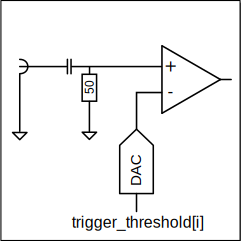
\includegraphics[width=0.3\textwidth]{xhptdc/figures/InputCircuit.pdf}
					}{
						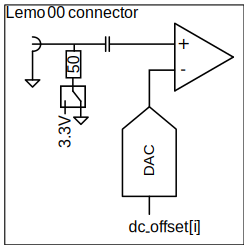
\includegraphics[width=0.3\textwidth]{figures/InputCircuit.pdf}
					}
					\caption{Input circuit for each of the input channels. \label{fig:dcoffset1}}
				\end{center} 
			\end{figure}
%%			\begin{figure}
%%				\begin{center}
%%					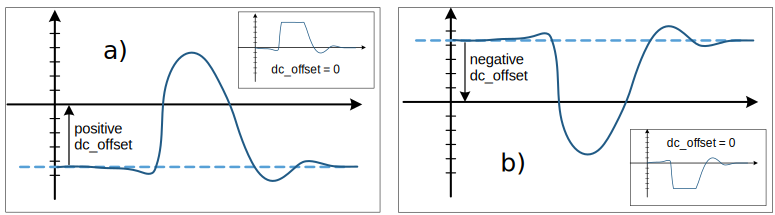
\includegraphics[width=\textwidth]{figures/dc_offset.pdf}
%%%					\caption{\textit{dc\tu offset} is used to shift the signal on each input channel such that the noise margin relative to the switching threshold is maximized.
%%					Insets of figure a) and b) show the base line of the signal with $\mathrm{\textit{dc\tu offset}}~=~0$ close to the switching threshold of the input buffer. Figure a) shows the positive pulse with $\mathrm{\textit{dc\tu offset}}~>~0$ and figure b) shows the negative pulse with $\mathrm{\textit{dc\tu offset}}~<~0$.\label{fig:dcoffset2}}
%%				\end{center}
%%			\end{figure}

			\ttvar{\prefix trigger}{trigger[\PREFIX TRIGGER\tu COUNT]}\\
			Configuration the polarity of the external trigger sources.
			These are used as inputs for the TiGer blocks and as inputs to the time measurement unit.\par

			\ttvar{\prefix tiger\tu block}{tiger\tu block[\PREFIX TIGER\tu COUNT]}
			Configuration of the timing generator (TiGer).

			\ttvar{\prefix channel}{channel[\PREFIX CHANNEL\tu COUNT]}\\
				Configure the TDC channels.

			\ttvar{\prefix low-res\tu channel}{low-res\tu channel[\PREFIX LOWRES\tu CHANNEL\tu COUNT]}\\
			\itett{
				Not applicable for \deviceName. 
			}{
				Only applicable to the xTDC4-Sciex. Configures the additional digital low-res inputs.
			}\par

			\cronvar{int}{auto\tu trigger\tu period}\\
			\cronvar{int}{auto\tu trigger\tu random\tu exponent}\\
			Create a trigger either periodically or randomly. There are two parameters $M = \text{trigger\tu period}$ and $N = \text{random\tu exponent}$ that result in a distance between triggers of $T$ clock cycles.

			\begin{align}
				T &= 1 + M + [1...2^N]\\
				&0 \leq M < 2^{32}\\
				&0 \leq N < 32
			\end{align}

			\noindent There is no enable or reset as the usage of this trigger can be configured in the TiGer block channel source field.\par

			\subsection{Structure \prefix trigger}
			\label{structtrigger}
			\cronvar{crono\tu bool\tu t}{falling}\\
			\cronvar{crono\tu bool\tu t}{rising}\\
			Select for which edges a trigger event is created inside the FPGA.
			\itett{
				The \deviceName can output measurements for one or both edges of input signals. 
			}{
				The \deviceName can output measurements with a reduced bin size of $5/6~ns = 833,\overline{3}~ps$ for one or both edges of input signals. 
				See section \ref{difficulthits} for more information on hits with varying resolution.
				Use \textsf{xtdc4\tu channel.rising} on page \pageref{structchannel} to select which edge is measured with full resolution.
				The edge that is selected for full resolution measurement must also be enabled for low resolution measurement.
			}\par

%%%%% tiger_block			

			\subsection{Structure \prefix tiger\tu block\label{cp:tigerblock}}

			\ifxHPTDC{
				\cronvar{int}{mode}\\
				Enables the desired mode of operation for the tiger.

				\begin{tabular}{lrl}
					\ttdef{TIGER \tu OFF} & 0 & no operation \\
					\ttdef{TIGER \tu OUTPUT} & 1 & output is driven with 2V amplitude. There must be no input connected \\
					\ttdef{TIGER \tu BIDI} & 2 & output is driven with 1V amplitude. Pulse rate should be low. \\
					\ttdef{TIGER \tu BIDI} & 2 & output is driven wuth 1V bidirectional pulses. $start = stop -1$\\
				\end{tabular}

				Gating blocks interpret any value that is not \ttdef{TIGER \tu OFF} as enable.	
			}{
				\cronvar{crono\tu bool\tu t}{enable}\\
				Activates the timing generator (TiGer).\par
			}
	
			\cronvar{crono\tu bool\tu t}{negate}\\
			Inverts output polarity. Default is set to false.
			\ifxHPTDC{For gating blocks, a value of false blocks inputs between start and stop, a value of true blocks outputs outside that interval.}{}\par
	
			\cronvar{crono\tu bool\tu t}{retrigger}\\
			Enables retrigger setting.\\
			If enabled the timer is reset to the value of the \textsf{start} parameter, whenever the input signal is set while waiting to reach the \textsf{stop} time.\par
	
			\cronvar{crono\tu bool\tu t}{extend}\\
			Not implemented.
	
			\ifxHPTDC{}{
				\cronvar{crono\tu bool\tu t}{enable\tu lemo\tu output}\\
				Enables the LEMO output. Drive the TiGer Signal to the corresponding Lemo connector as an output. 
				This is DC coupled, so make sure that you do not any devices connected as inputs.
				Pulses created by the TiGer are visible at the \deviceName inputs and can be measured again to get the exact timing.  
			}

			\cronvar{int}{start}\\
			\cronvar{int}{stop}\\
			\itett{
				In multiples of $4~ns$.
			}{
				In multiples of $20/3 = 6,\overline{6}~ns$
			}
			The time during which the TiGer output is set, relative to the trigger input. The parameters \textsf{start} and \textsf{stop} must fulfill the following conditions:
			\[ 0 <= start <= stop <= 2^{16}-1 \]
			If retriggering is enabled, the timer is reset to the value of the start parameter whenever the input signal is set while waiting for the stop time. \par
			
	
			\cronvar{int}{sources}\\
			A bit mask with a bit set for all trigger sources that can trigger this TiGer block. 
			Default is \textsf{\PREFIX TRIGGER\tu SOURCE\tu S}.\par
	
			\begin{tabular}{lc}
					 \ttdef{TRIGGER\tu SOURCE\tu S} & 0x00000001\\
					 \ttdef{TRIGGER\tu SOURCE\tu A} & 0x00000002\\
					 \ttdef{TRIGGER\tu SOURCE\tu B} & 0x00000004\\
					 \ttdef{TRIGGER\tu SOURCE\tu C} & 0x00000008\\
					 \ttdef{TRIGGER\tu SOURCE\tu D} & 0x00000010\\
					% \ttdef{TRIGGER\tu SOURCE\tu S1} & 0x00000020\\
					% \ttdef{TRIGGER\tu SOURCE\tu S2} & 0x00000040\\
					% \ttdef{TRIGGER\tu SOURCE\tu GATE} & 0x00000080\\
					 \ttdef{TRIGGER\tu SOURCE\tu AUTO} & 0x00004000\\
					 \ttdef{TRIGGER\tu SOURCE\tu ONE} & 0x00008000
				\end{tabular} 
	
			\subsection{Structure \prefix channel}
				\label{structchannel}
				Contains TDC channel settings.\par
	
				\cronvar{crono\tu bool\tu t}{enabled}\\
				Enable TDC channel.\par
	
				\cronvar{crono\tu bool\tu t}{rising}\\
				\itett{
					Not applicable for \deviceName.
				}{
					Select which edge of the signal is used for full resolution measurements. 
					\textsf{xtdc4\tu trigger.rising} and \textsf{xtdc4\tu trigger.falling} described on page \pageref{structtrigger} are used 
					to select which edges are recorded for low resolution measurement. 
					The edge that is selected for full resolution measurement must also be enabled for low resolution measurement.
					See section \ref{difficulthits} for more information on hits with varying resolution.
				}\par

				\itett{}{ % onyl for xTDC4
					\cronvar{crono\tu bool\tu t}{cc\tu enable}\\
					Enable carry chain TDC. This is set to \emph{true} by default and should be left unchanged. \par
	
					\cronvar{crono\tu bool\tu t}{cc\tu same\tu edge}\\
					Sets whether the carry chain TDC records the same or opposite edge as the TDC chip. 
					If the same edge is selected, that carry chain TDC acts  as a backup if the chip misses hits due to FIFO overflows or short input pulses.
					If opposite edges are selected, both edges of a pulse can be measured with reasonable resolution. See section \ref{difficulthits} for more information.\par
	
					\cronvar{crono\tu bool\tu t}{ths788\tu disable}\\
					Disable full resolution timestamps. This is set to \emph{false} by default and should be left unchanged.\par
				}
	
				\cronvar{int}{start}\\
				\cronvar{int}{stop}\\
				Veto function for grouping of hits into packets in multiples of the binsize. Only hits between start and stop are read out.
				The parameters must adhere to the following relations:
				\[
					0 <= start <= stop < 2^{ \itett{31}{30}}
				\]
	
	

	\section{Run Time Control}

			\ttvar{int}{continue\tu capture(}\ttvar{\prefix device}{*device)}\\
			Call this to resume data acquisition after a call to \textsf{\prefix pause\tu capture()}.\par

			\ttvar{int}{pause\tu capture(}\ttvar{\prefix device}{*device)}\\
			Pause data acquisition.\par

			\ttvar{int}{start\tu capture(}\ttvar{\prefix device}{*device)}\\
			Start data acquisition.\par

			\ttvar{int}{start\tu tiger(\ttvar{\prefix device}{*device})}\\
			Start timing generator.\par

			\ttvar{int}{stop\tu capture(}\ttvar{\prefix device}{*device)}\\
			Stop data acquisition.\par

			\ttvar{int}{stop\tu tiger(\ttvar{\prefix device}{*device})}\\
			Stop timing generator.\par

	\section{Readout\label{cp:readout}}

		\ttvar{int}{acknowledge(}\cronvar{\prefix device}{*device,} \cronvar{crono\tu packet}{*packet)}\\
		Acknowledges the processing of the last read block. This is only necessary if \textsf{\prefix read()} is not called with 
		\textsf{in.acknowledge\tu last\tu read} set.\\
		This feature allows to either free up partial DMA space early if there will be no call to \textsf{\prefix read()} anytime soon. 
		It also allows to keep data over multiple calls to \textsf{\prefix read()} to avoid unnecessary copying of data. \par

		\ttvar{int}{get\tu device\tu type}\\
		Returns the type of the device as \textsf{CRONO\tu DEVICE\tu \itett{TIMETAGGER4}{XTDC4}}.\par

		\ttvar{const char*}{get\tu last\tu error\tu message(\cronvar{\prefix device}{*device})}\\
		Returns most recent error message.\par

		\ttvar{int}{read(}\cronvar{\prefix device}{*device,} \cronvar{\prefix read\tu in}{*in,} \\ \cronvar{\prefix read\tu out}{*out)}\\
		Return a pointer to an array of captured data in \textsf{read\tu out}. 
		The result can contain any number of packets of type \textsf{\prefix packet}.
		\textsf{read\tu in} provides parameters to the driver. 
		A call to this method automatically allows the driver to reuse the memory returned in the previous call if \textsf{read\tu in.acknowledge\tu last\tu read} is set.\\
		Returns an error code as defined in the structure \textsf{\prefix read\tu out}.

		\subsection{Input Structure \prefix read\tu in}

			\ttvar{\prefix bool\tu t}{acknowledge\tu last\tu read}\\
			If set \textsf{\prefix read()} automatically acknowledges packets from the last read.

		\subsection{Input Structure \prefix read\tu out}
			\cronvar{crono\tu packet}{*first\tu packet}\\
			Pointer to the first packet that was capture by the call of \textsf{\prefix read}.\par

			\cronvar{crono\tu packet}{*last\tu packet}\\
			Address of header of the last packet in the buffer.\par

			\cronvar{int}{error\tu code}\\
			Assignments of the error codes.\par
			\begin{tabular}{lc}
				\crondef{CRONO\tu READ\tu OK} & 0\\
				\crondef{CRONO\tu READ\tu NO\tu DATA} & 1\\
				\crondef{CRONO\tu READ\tu INTERNAL\tu ERROR} & 2\\
				\crondef{CRONO\tu READ\tu TIMEOUT} & 3\par
			\end{tabular}\par

			\cronvar{const char}{*error\tu message}
			The last error in human readable form, possibly with additional information on the error.